\documentclass[twoside]{book}

% Packages required by doxygen
\usepackage{fixltx2e}
\usepackage{calc}
\usepackage{doxygen}
\usepackage[export]{adjustbox} % also loads graphicx
\usepackage{graphicx}
\usepackage[utf8]{inputenc}
\usepackage{makeidx}
\usepackage{multicol}
\usepackage{multirow}
\PassOptionsToPackage{warn}{textcomp}
\usepackage{textcomp}
\usepackage[nointegrals]{wasysym}
\usepackage[table]{xcolor}

% Font selection
\usepackage[T1]{fontenc}
\usepackage[scaled=.90]{helvet}
\usepackage{courier}
\usepackage{amssymb}
\usepackage{sectsty}
\renewcommand{\familydefault}{\sfdefault}
\allsectionsfont{%
  \fontseries{bc}\selectfont%
  \color{darkgray}%
}
\renewcommand{\DoxyLabelFont}{%
  \fontseries{bc}\selectfont%
  \color{darkgray}%
}
\newcommand{\+}{\discretionary{\mbox{\scriptsize$\hookleftarrow$}}{}{}}

% Page & text layout
\usepackage{geometry}
\geometry{%
  a4paper,%
  top=2.5cm,%
  bottom=2.5cm,%
  left=2.5cm,%
  right=2.5cm%
}
\tolerance=750
\hfuzz=15pt
\hbadness=750
\setlength{\emergencystretch}{15pt}
\setlength{\parindent}{0cm}
\setlength{\parskip}{0.2cm}
\makeatletter
\renewcommand{\paragraph}{%
  \@startsection{paragraph}{4}{0ex}{-1.0ex}{1.0ex}{%
    \normalfont\normalsize\bfseries\SS@parafont%
  }%
}
\renewcommand{\subparagraph}{%
  \@startsection{subparagraph}{5}{0ex}{-1.0ex}{1.0ex}{%
    \normalfont\normalsize\bfseries\SS@subparafont%
  }%
}
\makeatother

% Headers & footers
\usepackage{fancyhdr}
\pagestyle{fancyplain}
\fancyhead[LE]{\fancyplain{}{\bfseries\thepage}}
\fancyhead[CE]{\fancyplain{}{}}
\fancyhead[RE]{\fancyplain{}{\bfseries\leftmark}}
\fancyhead[LO]{\fancyplain{}{\bfseries\rightmark}}
\fancyhead[CO]{\fancyplain{}{}}
\fancyhead[RO]{\fancyplain{}{\bfseries\thepage}}
\fancyfoot[LE]{\fancyplain{}{}}
\fancyfoot[CE]{\fancyplain{}{}}
\fancyfoot[RE]{\fancyplain{}{\bfseries\scriptsize Generated on Thu Feb 19 2015 20\+:00\+:19 for My Project by Doxygen }}
\fancyfoot[LO]{\fancyplain{}{\bfseries\scriptsize Generated on Thu Feb 19 2015 20\+:00\+:19 for My Project by Doxygen }}
\fancyfoot[CO]{\fancyplain{}{}}
\fancyfoot[RO]{\fancyplain{}{}}
\renewcommand{\footrulewidth}{0.4pt}
\renewcommand{\chaptermark}[1]{%
  \markboth{#1}{}%
}
\renewcommand{\sectionmark}[1]{%
  \markright{\thesection\ #1}%
}

% Indices & bibliography
\usepackage{natbib}
\usepackage[titles]{tocloft}
\setcounter{tocdepth}{3}
\setcounter{secnumdepth}{5}
\makeindex

% Hyperlinks (required, but should be loaded last)
\usepackage{ifpdf}
\ifpdf
  \usepackage[pdftex,pagebackref=true]{hyperref}
\else
  \usepackage[ps2pdf,pagebackref=true]{hyperref}
\fi
\hypersetup{%
  colorlinks=true,%
  linkcolor=blue,%
  citecolor=blue,%
  unicode%
}

% Custom commands
\newcommand{\clearemptydoublepage}{%
  \newpage{\pagestyle{empty}\cleardoublepage}%
}


%===== C O N T E N T S =====

\begin{document}

% Titlepage & ToC
\hypersetup{pageanchor=false,
             bookmarks=true,
             bookmarksnumbered=true,
             pdfencoding=unicode
            }
\pagenumbering{roman}
\begin{titlepage}
\vspace*{7cm}
\begin{center}%
{\Large My Project }\\
\vspace*{1cm}
{\large Generated by Doxygen 1.8.9.1}\\
\vspace*{0.5cm}
{\small Thu Feb 19 2015 20:00:19}\\
\end{center}
\end{titlepage}
\clearemptydoublepage
\tableofcontents
\clearemptydoublepage
\pagenumbering{arabic}
\hypersetup{pageanchor=true}

%--- Begin generated contents ---
\chapter{Hierarchical Index}
\section{Class Hierarchy}
This inheritance list is sorted roughly, but not completely, alphabetically\+:\begin{DoxyCompactList}
\item \contentsline{section}{chess\+\_\+core.\+chess\+\_\+game}{\pageref{classchess__core_1_1chess__game}}{}
\begin{DoxyCompactList}
\item \contentsline{section}{square\+\_\+eight\+\_\+chess.\+square\+\_\+eight\+\_\+board}{\pageref{classsquare__eight__chess_1_1square__eight__board}}{}
\end{DoxyCompactList}
\item \contentsline{section}{square\+\_\+eight\+\_\+chess.\+chess\+\_\+game\+Test}{\pageref{classsquare__eight__chess_1_1chess__gameTest}}{}
\item \contentsline{section}{chess\+\_\+core.\+chess\+\_\+piece}{\pageref{classchess__core_1_1chess__piece}}{}
\begin{DoxyCompactList}
\item \contentsline{section}{chess\+\_\+core.\+pawn}{\pageref{classchess__core_1_1pawn}}{}
\item \contentsline{section}{chess\+\_\+core.\+sliding\+\_\+chess\+\_\+piece}{\pageref{classchess__core_1_1sliding__chess__piece}}{}
\begin{DoxyCompactList}
\item \contentsline{section}{chess\+\_\+core.\+bishop}{\pageref{classchess__core_1_1bishop}}{}
\item \contentsline{section}{chess\+\_\+core.\+queen}{\pageref{classchess__core_1_1queen}}{}
\item \contentsline{section}{chess\+\_\+core.\+rook}{\pageref{classchess__core_1_1rook}}{}
\end{DoxyCompactList}
\item \contentsline{section}{chess\+\_\+core.\+stepping\+\_\+chess\+\_\+piece}{\pageref{classchess__core_1_1stepping__chess__piece}}{}
\begin{DoxyCompactList}
\item \contentsline{section}{chess\+\_\+core.\+king}{\pageref{classchess__core_1_1king}}{}
\item \contentsline{section}{chess\+\_\+core.\+knight}{\pageref{classchess__core_1_1knight}}{}
\end{DoxyCompactList}
\end{DoxyCompactList}
\item \contentsline{section}{chess\+\_\+core.\+piece\+\_\+type}{\pageref{enumchess__core_1_1piece__type}}{}
\item \contentsline{section}{chess\+\_\+core.\+chess\+\_\+game.\+player}{\pageref{classchess__core_1_1chess__game_1_1player}}{}
\item \contentsline{section}{chess\+\_\+core.\+player\+\_\+status}{\pageref{enumchess__core_1_1player__status}}{}
\item \contentsline{section}{chess\+\_\+core.\+team\+\_\+color}{\pageref{enumchess__core_1_1team__color}}{}
\end{DoxyCompactList}

\chapter{Class Index}
\section{Class List}
Here are the classes, structs, unions and interfaces with brief descriptions\+:\begin{DoxyCompactList}
\item\contentsline{section}{\hyperlink{classchess__core_1_1bishop}{chess\+\_\+core.\+bishop} }{\pageref{classchess__core_1_1bishop}}{}
\item\contentsline{section}{\hyperlink{classchess__core_1_1chess__game}{chess\+\_\+core.\+chess\+\_\+game} }{\pageref{classchess__core_1_1chess__game}}{}
\item\contentsline{section}{\hyperlink{classsquare__eight__chess_1_1chess__gameTest}{square\+\_\+eight\+\_\+chess.\+chess\+\_\+game\+Test} }{\pageref{classsquare__eight__chess_1_1chess__gameTest}}{}
\item\contentsline{section}{\hyperlink{classchess__core_1_1chess__piece}{chess\+\_\+core.\+chess\+\_\+piece} }{\pageref{classchess__core_1_1chess__piece}}{}
\item\contentsline{section}{\hyperlink{classchess__core_1_1king}{chess\+\_\+core.\+king} }{\pageref{classchess__core_1_1king}}{}
\item\contentsline{section}{\hyperlink{classchess__core_1_1knight}{chess\+\_\+core.\+knight} }{\pageref{classchess__core_1_1knight}}{}
\item\contentsline{section}{\hyperlink{classchess__core_1_1pawn}{chess\+\_\+core.\+pawn} }{\pageref{classchess__core_1_1pawn}}{}
\item\contentsline{section}{\hyperlink{enumchess__core_1_1piece__type}{chess\+\_\+core.\+piece\+\_\+type} }{\pageref{enumchess__core_1_1piece__type}}{}
\item\contentsline{section}{\hyperlink{classchess__core_1_1chess__game_1_1player}{chess\+\_\+core.\+chess\+\_\+game.\+player} }{\pageref{classchess__core_1_1chess__game_1_1player}}{}
\item\contentsline{section}{\hyperlink{enumchess__core_1_1player__status}{chess\+\_\+core.\+player\+\_\+status} }{\pageref{enumchess__core_1_1player__status}}{}
\item\contentsline{section}{\hyperlink{classchess__core_1_1queen}{chess\+\_\+core.\+queen} }{\pageref{classchess__core_1_1queen}}{}
\item\contentsline{section}{\hyperlink{classchess__core_1_1rook}{chess\+\_\+core.\+rook} }{\pageref{classchess__core_1_1rook}}{}
\item\contentsline{section}{\hyperlink{classchess__core_1_1sliding__chess__piece}{chess\+\_\+core.\+sliding\+\_\+chess\+\_\+piece} }{\pageref{classchess__core_1_1sliding__chess__piece}}{}
\item\contentsline{section}{\hyperlink{classsquare__eight__chess_1_1square__eight__board}{square\+\_\+eight\+\_\+chess.\+square\+\_\+eight\+\_\+board} }{\pageref{classsquare__eight__chess_1_1square__eight__board}}{}
\item\contentsline{section}{\hyperlink{classchess__core_1_1stepping__chess__piece}{chess\+\_\+core.\+stepping\+\_\+chess\+\_\+piece} }{\pageref{classchess__core_1_1stepping__chess__piece}}{}
\item\contentsline{section}{\hyperlink{enumchess__core_1_1team__color}{chess\+\_\+core.\+team\+\_\+color} }{\pageref{enumchess__core_1_1team__color}}{}
\end{DoxyCompactList}

\chapter{Class Documentation}
\hypertarget{classchess__core_1_1bishop}{}\section{chess\+\_\+core.\+bishop Class Reference}
\label{classchess__core_1_1bishop}\index{chess\+\_\+core.\+bishop@{chess\+\_\+core.\+bishop}}
Inheritance diagram for chess\+\_\+core.\+bishop\+:\begin{figure}[H]
\begin{center}
\leavevmode
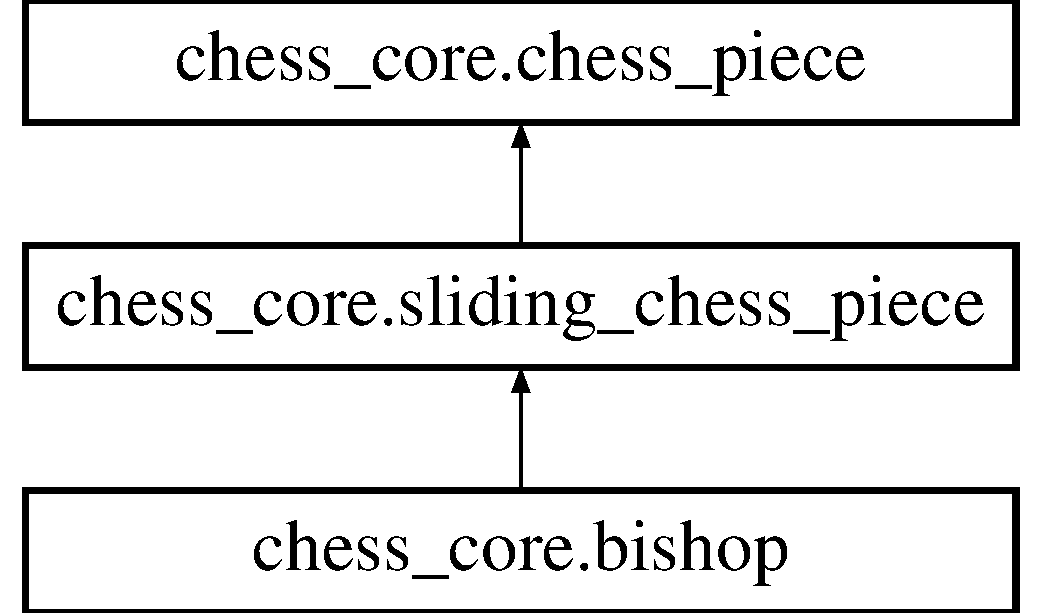
\includegraphics[height=3.000000cm]{classchess__core_1_1bishop}
\end{center}
\end{figure}
\subsection*{Public Member Functions}
\begin{DoxyCompactItemize}
\item 
\hypertarget{classchess__core_1_1bishop_a554ab5f785b4a94d3072cd6f4e598f1d}{}{\bfseries bishop} (Point starting\+\_\+pos, \hyperlink{enumchess__core_1_1team__color}{team\+\_\+color} team, \hyperlink{classchess__core_1_1chess__game}{chess\+\_\+game} board)\label{classchess__core_1_1bishop_a554ab5f785b4a94d3072cd6f4e598f1d}

\end{DoxyCompactItemize}
\subsection*{Additional Inherited Members}


\subsection{Detailed Description}
Created by tl on 2/11/15.

Nothing interesting here, extends sliding chess piece 

The documentation for this class was generated from the following file\+:\begin{DoxyCompactItemize}
\item 
src/chess\+\_\+core/bishop.\+java\end{DoxyCompactItemize}

\hypertarget{classchess__core_1_1chess__game}{}\section{chess\+\_\+core.\+chess\+\_\+game Class Reference}
\label{classchess__core_1_1chess__game}\index{chess\+\_\+core.\+chess\+\_\+game@{chess\+\_\+core.\+chess\+\_\+game}}
Inheritance diagram for chess\+\_\+core.\+chess\+\_\+game\+:\begin{figure}[H]
\begin{center}
\leavevmode
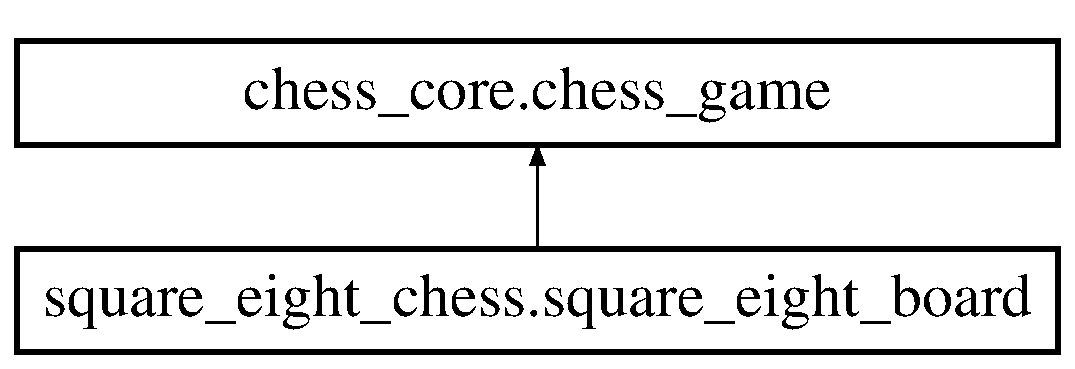
\includegraphics[height=2.000000cm]{classchess__core_1_1chess__game}
\end{center}
\end{figure}
\subsection*{Classes}
\begin{DoxyCompactItemize}
\item 
class \hyperlink{classchess__core_1_1chess__game_1_1player}{player}
\end{DoxyCompactItemize}
\subsection*{Public Member Functions}
\begin{DoxyCompactItemize}
\item 
\hypertarget{classchess__core_1_1chess__game_a99875295918d6625376849679319241b}{}abstract void {\bfseries init\+\_\+game} ()\label{classchess__core_1_1chess__game_a99875295918d6625376849679319241b}

\item 
\hypertarget{classchess__core_1_1chess__game_a9e94ac59c3ae17be159ce6c0df8e0274}{}abstract boolean {\bfseries is\+\_\+in\+\_\+bounds} (Point position)\label{classchess__core_1_1chess__game_a9e94ac59c3ae17be159ce6c0df8e0274}

\item 
\hypertarget{classchess__core_1_1chess__game_adbe4c11477e6944d8b2d5f593374849a}{}void {\bfseries update\+\_\+statuses} ()\label{classchess__core_1_1chess__game_adbe4c11477e6944d8b2d5f593374849a}

\item 
\hypertarget{classchess__core_1_1chess__game_a84ed035e51594ec6e4c52682e87307ac}{}{\bfseries chess\+\_\+game} (\hyperlink{classchess__core_1_1chess__game}{chess\+\_\+game} other)\label{classchess__core_1_1chess__game_a84ed035e51594ec6e4c52682e87307ac}

\item 
\hypertarget{classchess__core_1_1chess__game_a5ebd04c4b1b82ce5e26dbe1f8e18b1ce}{}void {\bfseries update\+\_\+all\+\_\+moves} ()\label{classchess__core_1_1chess__game_a5ebd04c4b1b82ce5e26dbe1f8e18b1ce}

\item 
\hypertarget{classchess__core_1_1chess__game_a3460924fb30b8f9a04ce25db76f124dc}{}void {\bfseries update\+\_\+board} (Point old\+\_\+position, Point new\+\_\+position, \hyperlink{classchess__core_1_1chess__piece}{chess\+\_\+piece} piece)\label{classchess__core_1_1chess__game_a3460924fb30b8f9a04ce25db76f124dc}

\item 
\hypertarget{classchess__core_1_1chess__game_a868b923e9dc89aa1bac92f108d99c769}{}void {\bfseries capture\+\_\+piece} (Point position)\label{classchess__core_1_1chess__game_a868b923e9dc89aa1bac92f108d99c769}

\item 
\hypertarget{classchess__core_1_1chess__game_a302ddb48ccde5fb6237c314dc5c2dce5}{}\hyperlink{enumchess__core_1_1team__color}{team\+\_\+color} {\bfseries get\+\_\+occupying\+\_\+color} (Point point)\label{classchess__core_1_1chess__game_a302ddb48ccde5fb6237c314dc5c2dce5}

\item 
\hypertarget{classchess__core_1_1chess__game_ae06f22607a25c2eb8506028bf36cd029}{}List$<$ Point $>$ {\bfseries get\+\_\+movelist} (Point point)\label{classchess__core_1_1chess__game_ae06f22607a25c2eb8506028bf36cd029}

\item 
\hypertarget{classchess__core_1_1chess__game_a148c8578eb1f84b6f14a73587ac6b232}{}boolean {\bfseries spot\+\_\+empty} (Point point)\label{classchess__core_1_1chess__game_a148c8578eb1f84b6f14a73587ac6b232}

\item 
\hypertarget{classchess__core_1_1chess__game_a5fddc69fb2cb29aa8ffd071c40289a11}{}List$<$ \hyperlink{classchess__core_1_1chess__piece}{chess\+\_\+piece} $>$ {\bfseries get\+\_\+player\+\_\+pieces} (\hyperlink{enumchess__core_1_1team__color}{team\+\_\+color} color)\label{classchess__core_1_1chess__game_a5fddc69fb2cb29aa8ffd071c40289a11}

\item 
\hypertarget{classchess__core_1_1chess__game_ab3a5f5c195645e86285d69895e51fd5d}{}\hyperlink{enumchess__core_1_1player__status}{player\+\_\+status} {\bfseries get\+\_\+player\+\_\+status} (\hyperlink{enumchess__core_1_1team__color}{team\+\_\+color} color)\label{classchess__core_1_1chess__game_ab3a5f5c195645e86285d69895e51fd5d}

\item 
\hypertarget{classchess__core_1_1chess__game_a9c144a5e9c141119dc8c3820b8d05d13}{}\hyperlink{classchess__core_1_1chess__piece}{chess\+\_\+piece} {\bfseries get\+\_\+piece\+\_\+at} (Point position)\label{classchess__core_1_1chess__game_a9c144a5e9c141119dc8c3820b8d05d13}

\item 
\hypertarget{classchess__core_1_1chess__game_a4efa1ef50e67b669c56cd482b8378f78}{}void {\bfseries move\+\_\+piece} (Point from, Point to)  throws Exception\label{classchess__core_1_1chess__game_a4efa1ef50e67b669c56cd482b8378f78}

\item 
\hypertarget{classchess__core_1_1chess__game_a57b8ea6545cf8dabeb00e05305a11520}{}void {\bfseries make\+\_\+piece} (int x, int y, \hyperlink{enumchess__core_1_1team__color}{team\+\_\+color} color, \hyperlink{enumchess__core_1_1piece__type}{piece\+\_\+type} type)\label{classchess__core_1_1chess__game_a57b8ea6545cf8dabeb00e05305a11520}

\item 
\hypertarget{classchess__core_1_1chess__game_af267d2fc681a90ea7afdaf49f7034c9f}{}void {\bfseries put\+\_\+piece} (\hyperlink{classchess__core_1_1chess__piece}{chess\+\_\+piece} piece, Point position)\label{classchess__core_1_1chess__game_af267d2fc681a90ea7afdaf49f7034c9f}

\item 
\hypertarget{classchess__core_1_1chess__game_adfded27abed79ceced263ce726c48a13}{}boolean {\bfseries is\+\_\+simulating} ()\label{classchess__core_1_1chess__game_adfded27abed79ceced263ce726c48a13}

\item 
\hypertarget{classchess__core_1_1chess__game_a2625d75d88e1ad39dec7d34f713d1c01}{}boolean {\bfseries simulate\+\_\+move\+\_\+safety} (\hyperlink{classchess__core_1_1chess__piece}{chess\+\_\+piece} piece, Point position)  throws Exception \label{classchess__core_1_1chess__game_a2625d75d88e1ad39dec7d34f713d1c01}

\end{DoxyCompactItemize}
\subsection*{Protected Attributes}
\begin{DoxyCompactItemize}
\item 
\hypertarget{classchess__core_1_1chess__game_ac61db7251fc43f61985873492b6aede9}{}Hash\+Map$<$ Point, \hyperlink{classchess__core_1_1chess__piece}{chess\+\_\+piece} $>$ {\bfseries board}\label{classchess__core_1_1chess__game_ac61db7251fc43f61985873492b6aede9}

\item 
\hypertarget{classchess__core_1_1chess__game_a8bd15d77a95a3e8aa05895925390b321}{}\hyperlink{classchess__core_1_1chess__game_1_1player}{player} {\bfseries black}\label{classchess__core_1_1chess__game_a8bd15d77a95a3e8aa05895925390b321}

\item 
\hypertarget{classchess__core_1_1chess__game_a8bfcc0cfb084ed368c9fcc667969e766}{}\hyperlink{classchess__core_1_1chess__game_1_1player}{player} {\bfseries white}\label{classchess__core_1_1chess__game_a8bfcc0cfb084ed368c9fcc667969e766}

\end{DoxyCompactItemize}


\subsection{Detailed Description}
Created by tl on 2/10/15.

chess game main class. an abstract class all chess games made should extend the \hyperlink{classchess__core_1_1chess__game}{chess\+\_\+core.\+chess\+\_\+game} class, which contains the logic involved for the main functions

to make a custom chess game (completely extensible) implement the following two functions\+:
\begin{DoxyItemize}
\item init\+\_\+game() -\/ tell the game what pieces to put and where on the board
\item is\+\_\+in\+\_\+bounds(\+Point position) tells the game what \char`\"{}parts\char`\"{} of the board are in bounds all functions used to determine activity will determine if a move is legal by calling this function 
\end{DoxyItemize}

The documentation for this class was generated from the following file\+:\begin{DoxyCompactItemize}
\item 
src/chess\+\_\+core/chess\+\_\+game.\+java\end{DoxyCompactItemize}

\hypertarget{classsquare__eight__chess_1_1chess__gameTest}{}\section{square\+\_\+eight\+\_\+chess.\+chess\+\_\+game\+Test Class Reference}
\label{classsquare__eight__chess_1_1chess__gameTest}\index{square\+\_\+eight\+\_\+chess.\+chess\+\_\+game\+Test@{square\+\_\+eight\+\_\+chess.\+chess\+\_\+game\+Test}}
\subsection*{Public Member Functions}
\begin{DoxyCompactItemize}
\item 
\hypertarget{classsquare__eight__chess_1_1chess__gameTest_aa466120f1d3931fd2baaa56df8b11cfc}{}void {\bfseries test\+Init\+\_\+game} ()  throws Exception \label{classsquare__eight__chess_1_1chess__gameTest_aa466120f1d3931fd2baaa56df8b11cfc}

\item 
\hypertarget{classsquare__eight__chess_1_1chess__gameTest_a53b86c51b64c5d4653a04d58918a3293}{}void {\bfseries test\+\_\+move\+\_\+pawn} ()  throws Exception \label{classsquare__eight__chess_1_1chess__gameTest_a53b86c51b64c5d4653a04d58918a3293}

\item 
\hypertarget{classsquare__eight__chess_1_1chess__gameTest_a79f78d1f8c78665feae66b947a3687cb}{}void {\bfseries test\+\_\+capturing} ()  throws Exception \label{classsquare__eight__chess_1_1chess__gameTest_a79f78d1f8c78665feae66b947a3687cb}

\item 
\hypertarget{classsquare__eight__chess_1_1chess__gameTest_a8708ed5fc7c5490db86ce20158fca416}{}void {\bfseries test\+\_\+bishop} ()  throws Exception \label{classsquare__eight__chess_1_1chess__gameTest_a8708ed5fc7c5490db86ce20158fca416}

\item 
\hypertarget{classsquare__eight__chess_1_1chess__gameTest_af616e72ebfd8b9ddc5f954a3dbc25786}{}void {\bfseries test\+\_\+illegal\+\_\+move} ()  throws Exception \label{classsquare__eight__chess_1_1chess__gameTest_af616e72ebfd8b9ddc5f954a3dbc25786}

\item 
\hypertarget{classsquare__eight__chess_1_1chess__gameTest_ac7a16595bfb5f4472566a788605e3be1}{}void {\bfseries test\+\_\+rook} ()  throws Exception \label{classsquare__eight__chess_1_1chess__gameTest_ac7a16595bfb5f4472566a788605e3be1}

\item 
\hypertarget{classsquare__eight__chess_1_1chess__gameTest_ab4b66c800b00adc8779de0c8939a9a61}{}void {\bfseries test\+\_\+queen} ()  throws Exception \label{classsquare__eight__chess_1_1chess__gameTest_ab4b66c800b00adc8779de0c8939a9a61}

\item 
\hypertarget{classsquare__eight__chess_1_1chess__gameTest_a9f7b3f5296115fc1a9853da259042932}{}void {\bfseries test\+\_\+knight} ()  throws Exception \label{classsquare__eight__chess_1_1chess__gameTest_a9f7b3f5296115fc1a9853da259042932}

\item 
\hypertarget{classsquare__eight__chess_1_1chess__gameTest_a167930c1a9b5353fd0c0abb6892b79f6}{}void {\bfseries test\+\_\+king} ()  throws Exception \label{classsquare__eight__chess_1_1chess__gameTest_a167930c1a9b5353fd0c0abb6892b79f6}

\item 
\hypertarget{classsquare__eight__chess_1_1chess__gameTest_ab6b0d2fe1bf4f49c89deb32eece458c2}{}void {\bfseries test\+\_\+checkedness} ()  throws Exception \label{classsquare__eight__chess_1_1chess__gameTest_ab6b0d2fe1bf4f49c89deb32eece458c2}

\item 
\hypertarget{classsquare__eight__chess_1_1chess__gameTest_abffaf55ec4431e93db1bf53dd045f4e9}{}void {\bfseries test\+\_\+checkmate} ()  throws Exception \label{classsquare__eight__chess_1_1chess__gameTest_abffaf55ec4431e93db1bf53dd045f4e9}

\end{DoxyCompactItemize}


The documentation for this class was generated from the following file\+:\begin{DoxyCompactItemize}
\item 
src/square\+\_\+eight\+\_\+chess/chess\+\_\+game\+Test.\+java\end{DoxyCompactItemize}

\hypertarget{classchess__core_1_1chess__piece}{}\section{chess\+\_\+core.\+chess\+\_\+piece Class Reference}
\label{classchess__core_1_1chess__piece}\index{chess\+\_\+core.\+chess\+\_\+piece@{chess\+\_\+core.\+chess\+\_\+piece}}
Inheritance diagram for chess\+\_\+core.\+chess\+\_\+piece\+:\begin{figure}[H]
\begin{center}
\leavevmode
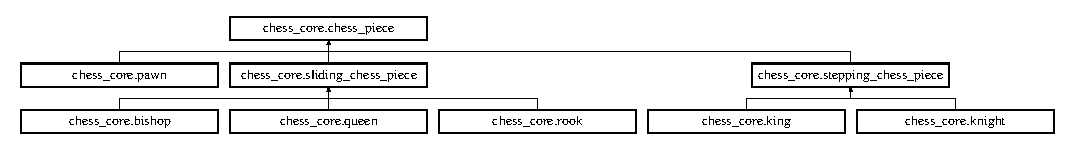
\includegraphics[height=1.562791cm]{classchess__core_1_1chess__piece}
\end{center}
\end{figure}
\subsection*{Public Member Functions}
\begin{DoxyCompactItemize}
\item 
\hypertarget{classchess__core_1_1chess__piece_ae20fe8201ff79d7fcbc6f80fa6315fc4}{}{\bfseries chess\+\_\+piece} (Point starting\+\_\+pos, \hyperlink{enumchess__core_1_1team__color}{team\+\_\+color} team, \hyperlink{classchess__core_1_1chess__game}{chess\+\_\+game} board)\label{classchess__core_1_1chess__piece_ae20fe8201ff79d7fcbc6f80fa6315fc4}

\item 
\hypertarget{classchess__core_1_1chess__piece_a06a36898ea2909b718ddd001ef0386ac}{}void {\bfseries move\+\_\+piece} (Point new\+\_\+position)  throws Exception\label{classchess__core_1_1chess__piece_a06a36898ea2909b718ddd001ef0386ac}

\item 
\hypertarget{classchess__core_1_1chess__piece_aa7f23946622ad63461492d95f5fb095e}{}void {\bfseries simulate\+\_\+move} (Point new\+\_\+position)\label{classchess__core_1_1chess__piece_aa7f23946622ad63461492d95f5fb095e}

\item 
\hypertarget{classchess__core_1_1chess__piece_a80e2e675b899fa530b56c0670aec2c98}{}boolean {\bfseries add\+\_\+move} (Point point)\label{classchess__core_1_1chess__piece_a80e2e675b899fa530b56c0670aec2c98}

\item 
\hypertarget{classchess__core_1_1chess__piece_a92463a5265b949fccf53522da8230bc4}{}void {\bfseries safe\+\_\+add} (Point point)\label{classchess__core_1_1chess__piece_a92463a5265b949fccf53522da8230bc4}

\item 
\hypertarget{classchess__core_1_1chess__piece_ac726b474dc222bdb9a4a8043d5e4b203}{}\hyperlink{enumchess__core_1_1piece__type}{piece\+\_\+type} {\bfseries get\+\_\+type} ()\label{classchess__core_1_1chess__piece_ac726b474dc222bdb9a4a8043d5e4b203}

\item 
\hypertarget{classchess__core_1_1chess__piece_ab6b3ac1a35546681062effa03e9a2c5b}{}Point {\bfseries get\+\_\+position} ()\label{classchess__core_1_1chess__piece_ab6b3ac1a35546681062effa03e9a2c5b}

\item 
\hypertarget{classchess__core_1_1chess__piece_a71787594c92088a269afc5f36c280a36}{}List$<$ Point $>$ {\bfseries get\+\_\+possible\+\_\+moves} ()\label{classchess__core_1_1chess__piece_a71787594c92088a269afc5f36c280a36}

\item 
\hypertarget{classchess__core_1_1chess__piece_a05ecf4fad3195cb33a24f33b51c68738}{}\hyperlink{enumchess__core_1_1team__color}{team\+\_\+color} {\bfseries get\+\_\+team} ()\label{classchess__core_1_1chess__piece_a05ecf4fad3195cb33a24f33b51c68738}

\end{DoxyCompactItemize}
\subsection*{Protected Member Functions}
\begin{DoxyCompactItemize}
\item 
\hypertarget{classchess__core_1_1chess__piece_a884b073a0e40e68bf0e1a670df307755}{}abstract void {\bfseries update\+\_\+possible\+\_\+moves} ()\label{classchess__core_1_1chess__piece_a884b073a0e40e68bf0e1a670df307755}

\end{DoxyCompactItemize}
\subsection*{Protected Attributes}
\begin{DoxyCompactItemize}
\item 
\hypertarget{classchess__core_1_1chess__piece_ab8be2da54759e79e10ffc8ee3b391773}{}\hyperlink{enumchess__core_1_1piece__type}{piece\+\_\+type} {\bfseries type}\label{classchess__core_1_1chess__piece_ab8be2da54759e79e10ffc8ee3b391773}

\item 
\hypertarget{classchess__core_1_1chess__piece_af35cb6eadaebeebec1f6eff9d6db3c38}{}Point {\bfseries position}\label{classchess__core_1_1chess__piece_af35cb6eadaebeebec1f6eff9d6db3c38}

\item 
\hypertarget{classchess__core_1_1chess__piece_a09d4544e8fc841454daafc9cdb29ca6c}{}List$<$ Point $>$ {\bfseries possible\+\_\+moves}\label{classchess__core_1_1chess__piece_a09d4544e8fc841454daafc9cdb29ca6c}

\item 
\hypertarget{classchess__core_1_1chess__piece_a828388a4dec818013f2fa78b2cb01b9c}{}\hyperlink{enumchess__core_1_1team__color}{team\+\_\+color} {\bfseries team}\label{classchess__core_1_1chess__piece_a828388a4dec818013f2fa78b2cb01b9c}

\item 
\hypertarget{classchess__core_1_1chess__piece_a1ede1fdde8149ddfea0056fc45ed5c71}{}\hyperlink{classchess__core_1_1chess__game}{chess\+\_\+game} {\bfseries chess\+\_\+board}\label{classchess__core_1_1chess__piece_a1ede1fdde8149ddfea0056fc45ed5c71}

\end{DoxyCompactItemize}


\subsection{Detailed Description}
Created by tl on 2/10/15.

Base class for the chess piece. abstract class All pieces should either extend chess piece or extend a subclass Current extendable subclasses \+: \hyperlink{classchess__core_1_1sliding__chess__piece}{chess\+\_\+core.\+sliding\+\_\+chess\+\_\+piece} and \hyperlink{classchess__core_1_1stepping__chess__piece}{chess\+\_\+core.\+stepping\+\_\+chess\+\_\+piece} (See respective classes) 

The documentation for this class was generated from the following file\+:\begin{DoxyCompactItemize}
\item 
src/chess\+\_\+core/chess\+\_\+piece.\+java\end{DoxyCompactItemize}

\hypertarget{classchess__core_1_1king}{}\section{chess\+\_\+core.\+king Class Reference}
\label{classchess__core_1_1king}\index{chess\+\_\+core.\+king@{chess\+\_\+core.\+king}}
Inheritance diagram for chess\+\_\+core.\+king\+:\begin{figure}[H]
\begin{center}
\leavevmode
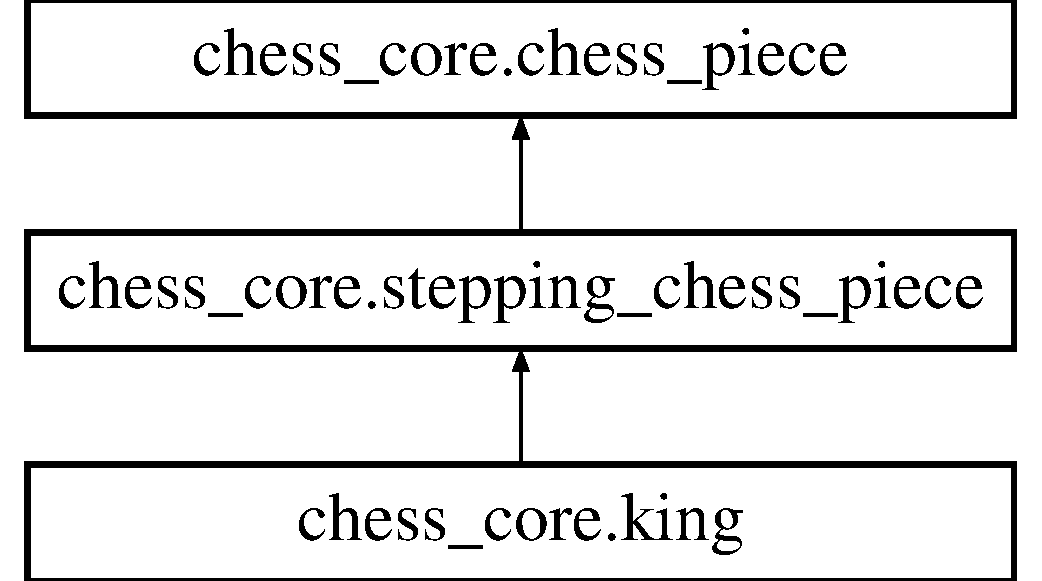
\includegraphics[height=3.000000cm]{classchess__core_1_1king}
\end{center}
\end{figure}
\subsection*{Public Member Functions}
\begin{DoxyCompactItemize}
\item 
\hypertarget{classchess__core_1_1king_a2005a51df2644082860009f9d0372ff3}{}{\bfseries king} (Point starting\+\_\+pos, \hyperlink{enumchess__core_1_1team__color}{team\+\_\+color} team, \hyperlink{classchess__core_1_1chess__game}{chess\+\_\+game} board)\label{classchess__core_1_1king_a2005a51df2644082860009f9d0372ff3}

\end{DoxyCompactItemize}
\subsection*{Additional Inherited Members}


\subsection{Detailed Description}
Created by tl on 2/11/15. Nothing interesting here, extends stepping chess piece 

The documentation for this class was generated from the following file\+:\begin{DoxyCompactItemize}
\item 
src/chess\+\_\+core/king.\+java\end{DoxyCompactItemize}

\hypertarget{classchess__core_1_1knight}{}\section{chess\+\_\+core.\+knight Class Reference}
\label{classchess__core_1_1knight}\index{chess\+\_\+core.\+knight@{chess\+\_\+core.\+knight}}
Inheritance diagram for chess\+\_\+core.\+knight\+:\begin{figure}[H]
\begin{center}
\leavevmode
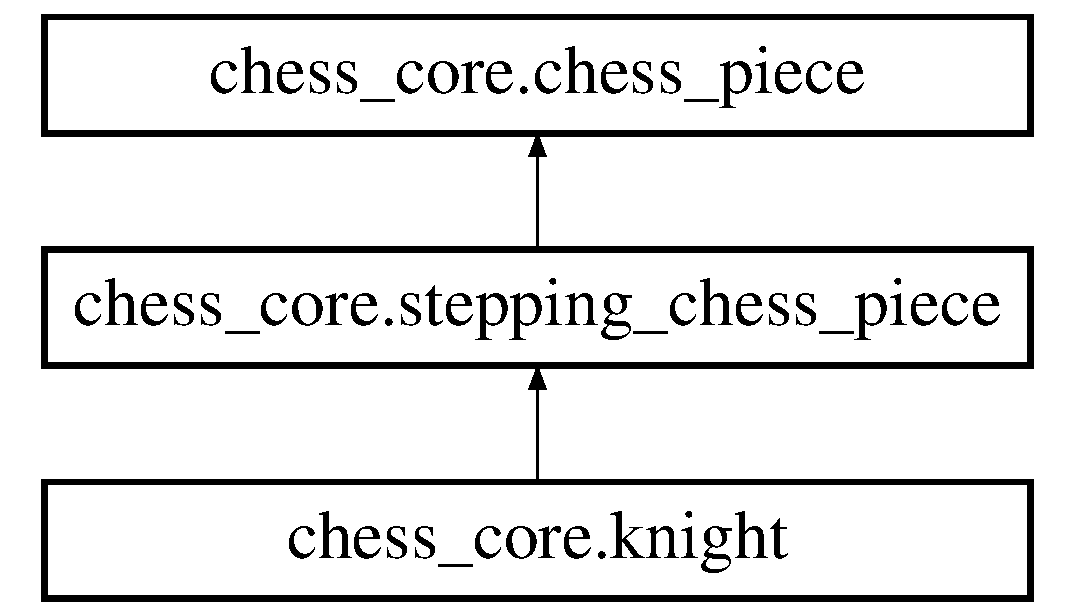
\includegraphics[height=3.000000cm]{classchess__core_1_1knight}
\end{center}
\end{figure}
\subsection*{Public Member Functions}
\begin{DoxyCompactItemize}
\item 
\hypertarget{classchess__core_1_1knight_aa6b9c2401b5f0c1e2642b2c57810b882}{}{\bfseries knight} (Point starting\+\_\+pos, \hyperlink{enumchess__core_1_1team__color}{team\+\_\+color} team, \hyperlink{classchess__core_1_1chess__game}{chess\+\_\+game} board)\label{classchess__core_1_1knight_aa6b9c2401b5f0c1e2642b2c57810b882}

\end{DoxyCompactItemize}
\subsection*{Additional Inherited Members}


\subsection{Detailed Description}
Created by tl on 2/11/15. Nothing interesting here, extends stepping chess piece 

The documentation for this class was generated from the following file\+:\begin{DoxyCompactItemize}
\item 
src/chess\+\_\+core/knight.\+java\end{DoxyCompactItemize}

\hypertarget{classchess__core_1_1pawn}{}\section{chess\+\_\+core.\+pawn Class Reference}
\label{classchess__core_1_1pawn}\index{chess\+\_\+core.\+pawn@{chess\+\_\+core.\+pawn}}
Inheritance diagram for chess\+\_\+core.\+pawn\+:\begin{figure}[H]
\begin{center}
\leavevmode
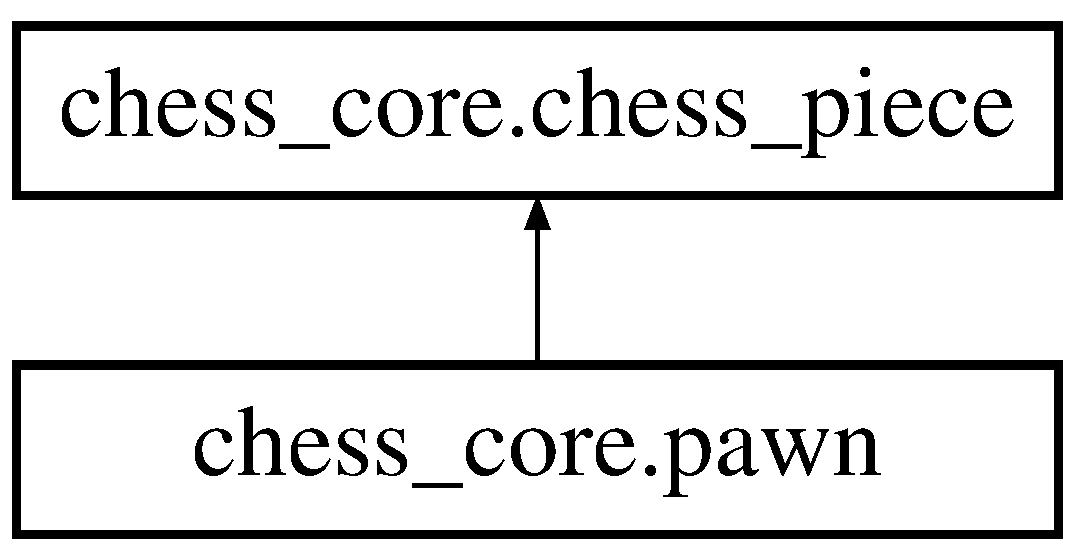
\includegraphics[height=2.000000cm]{classchess__core_1_1pawn}
\end{center}
\end{figure}
\subsection*{Public Member Functions}
\begin{DoxyCompactItemize}
\item 
\hypertarget{classchess__core_1_1pawn_a78b371273a0dee8542b32cb53b82776e}{}{\bfseries pawn} (Point starting\+\_\+pos, \hyperlink{enumchess__core_1_1team__color}{team\+\_\+color} team, \hyperlink{classchess__core_1_1chess__game}{chess\+\_\+game} board)\label{classchess__core_1_1pawn_a78b371273a0dee8542b32cb53b82776e}

\end{DoxyCompactItemize}
\subsection*{Protected Member Functions}
\begin{DoxyCompactItemize}
\item 
\hypertarget{classchess__core_1_1pawn_a12a53bd7aad2887e74754b7815f5d229}{}void {\bfseries update\+\_\+possible\+\_\+moves} ()\label{classchess__core_1_1pawn_a12a53bd7aad2887e74754b7815f5d229}

\end{DoxyCompactItemize}
\subsection*{Additional Inherited Members}


\subsection{Detailed Description}
Created by tl on 2/10/15. Nothing interesting here, extends chess piece 

The documentation for this class was generated from the following file\+:\begin{DoxyCompactItemize}
\item 
src/chess\+\_\+core/pawn.\+java\end{DoxyCompactItemize}

\hypertarget{enumchess__core_1_1piece__type}{}\section{chess\+\_\+core.\+piece\+\_\+type Enum Reference}
\label{enumchess__core_1_1piece__type}\index{chess\+\_\+core.\+piece\+\_\+type@{chess\+\_\+core.\+piece\+\_\+type}}
\subsection*{Public Attributes}
\begin{DoxyCompactItemize}
\item 
\hypertarget{enumchess__core_1_1piece__type_a427cc084c192a5499565270fd5e3ddc1}{}{\bfseries Rook}\label{enumchess__core_1_1piece__type_a427cc084c192a5499565270fd5e3ddc1}

\item 
\hypertarget{enumchess__core_1_1piece__type_a7349952c1bcc5dcfc59d3d713e9f0a60}{}{\bfseries Bishop}\label{enumchess__core_1_1piece__type_a7349952c1bcc5dcfc59d3d713e9f0a60}

\item 
\hypertarget{enumchess__core_1_1piece__type_a652ab261ad39276e67b8c8f6cd537e1c}{}{\bfseries Knight}\label{enumchess__core_1_1piece__type_a652ab261ad39276e67b8c8f6cd537e1c}

\item 
\hypertarget{enumchess__core_1_1piece__type_a2cef34c95f682b292c9d60b0266e6c34}{}{\bfseries King}\label{enumchess__core_1_1piece__type_a2cef34c95f682b292c9d60b0266e6c34}

\item 
\hypertarget{enumchess__core_1_1piece__type_adab30e670a64d0505076a2ccfcc36980}{}{\bfseries Queen}\label{enumchess__core_1_1piece__type_adab30e670a64d0505076a2ccfcc36980}

\item 
\hypertarget{enumchess__core_1_1piece__type_ab31ceb7e41830bfbe64f5da564caaaf4}{}{\bfseries Pawn}\label{enumchess__core_1_1piece__type_ab31ceb7e41830bfbe64f5da564caaaf4}

\end{DoxyCompactItemize}


\subsection{Detailed Description}
Created by tl on 2/10/15. enums for the makeable types 

The documentation for this enum was generated from the following file\+:\begin{DoxyCompactItemize}
\item 
src/chess\+\_\+core/piece\+\_\+type.\+java\end{DoxyCompactItemize}

\hypertarget{classchess__core_1_1chess__game_1_1player}{}\section{chess\+\_\+core.\+chess\+\_\+game.\+player Class Reference}
\label{classchess__core_1_1chess__game_1_1player}\index{chess\+\_\+core.\+chess\+\_\+game.\+player@{chess\+\_\+core.\+chess\+\_\+game.\+player}}
\subsection*{Public Member Functions}
\begin{DoxyCompactItemize}
\item 
\hypertarget{classchess__core_1_1chess__game_1_1player_ab932b0747af832c8e294f7dc0a34543a}{}{\bfseries player} (\hyperlink{enumchess__core_1_1team__color}{team\+\_\+color} color)\label{classchess__core_1_1chess__game_1_1player_ab932b0747af832c8e294f7dc0a34543a}

\item 
\hypertarget{classchess__core_1_1chess__game_1_1player_ae1f662d1ab3b8fe53e21545fc5e2b671}{}void {\bfseries set\+\_\+status} (\hyperlink{enumchess__core_1_1player__status}{player\+\_\+status} new\+\_\+status)\label{classchess__core_1_1chess__game_1_1player_ae1f662d1ab3b8fe53e21545fc5e2b671}

\item 
\hypertarget{classchess__core_1_1chess__game_1_1player_a8613ebf856946ba911073f3c1d20a3b4}{}void {\bfseries capture\+\_\+piece} (\hyperlink{classchess__core_1_1chess__piece}{chess\+\_\+piece} piece)\label{classchess__core_1_1chess__game_1_1player_a8613ebf856946ba911073f3c1d20a3b4}

\item 
\hypertarget{classchess__core_1_1chess__game_1_1player_afd9d550f13050d9ea3d0c2f3b91ce74a}{}void {\bfseries add\+\_\+piece} (\hyperlink{classchess__core_1_1chess__piece}{chess\+\_\+piece} piece)\label{classchess__core_1_1chess__game_1_1player_afd9d550f13050d9ea3d0c2f3b91ce74a}

\item 
\hypertarget{classchess__core_1_1chess__game_1_1player_a6b2e489c5a8764e0b9948034d003efde}{}void {\bfseries flip\+\_\+turn} ()\label{classchess__core_1_1chess__game_1_1player_a6b2e489c5a8764e0b9948034d003efde}

\item 
\hypertarget{classchess__core_1_1chess__game_1_1player_a40a2c16b2a5ce09fa323fe8989fd9d5a}{}\hyperlink{enumchess__core_1_1player__status}{player\+\_\+status} {\bfseries get\+\_\+status} ()\label{classchess__core_1_1chess__game_1_1player_a40a2c16b2a5ce09fa323fe8989fd9d5a}

\item 
\hypertarget{classchess__core_1_1chess__game_1_1player_af05cb913814162b672d107e40bb2bc45}{}void {\bfseries checkmate\+\_\+check} ()\label{classchess__core_1_1chess__game_1_1player_af05cb913814162b672d107e40bb2bc45}

\item 
\hypertarget{classchess__core_1_1chess__game_1_1player_a703c3b61a03ad5bd3301ffe100f3dd90}{}void {\bfseries update\+\_\+all\+\_\+moves} ()\label{classchess__core_1_1chess__game_1_1player_a703c3b61a03ad5bd3301ffe100f3dd90}

\item 
\hypertarget{classchess__core_1_1chess__game_1_1player_a9339ace043de1a8e0b99817ed9bf2bc1}{}\hyperlink{classchess__core_1_1chess__piece}{chess\+\_\+piece} {\bfseries get\+\_\+king} ()\label{classchess__core_1_1chess__game_1_1player_a9339ace043de1a8e0b99817ed9bf2bc1}

\item 
\hypertarget{classchess__core_1_1chess__game_1_1player_a53968bd363049db699f352b1c02bdc1d}{}boolean {\bfseries spot\+\_\+is\+\_\+covered} (Point position)\label{classchess__core_1_1chess__game_1_1player_a53968bd363049db699f352b1c02bdc1d}

\item 
\hypertarget{classchess__core_1_1chess__game_1_1player_a68aeb81dc6b94c95dff92c75facba1ba}{}List$<$ \hyperlink{classchess__core_1_1chess__piece}{chess\+\_\+piece} $>$ {\bfseries get\+\_\+pieces} ()\label{classchess__core_1_1chess__game_1_1player_a68aeb81dc6b94c95dff92c75facba1ba}

\end{DoxyCompactItemize}


The documentation for this class was generated from the following file\+:\begin{DoxyCompactItemize}
\item 
src/chess\+\_\+core/chess\+\_\+game.\+java\end{DoxyCompactItemize}

\hypertarget{enumchess__core_1_1player__status}{}\section{chess\+\_\+core.\+player\+\_\+status Enum Reference}
\label{enumchess__core_1_1player__status}\index{chess\+\_\+core.\+player\+\_\+status@{chess\+\_\+core.\+player\+\_\+status}}
\subsection*{Public Attributes}
\begin{DoxyCompactItemize}
\item 
\hypertarget{enumchess__core_1_1player__status_a37022bc4f450aa36df0b3fd9c4f15ca3}{}{\bfseries Safe}\label{enumchess__core_1_1player__status_a37022bc4f450aa36df0b3fd9c4f15ca3}

\item 
\hypertarget{enumchess__core_1_1player__status_a24548feb398c78cc6f423db107c7c163}{}{\bfseries Checked}\label{enumchess__core_1_1player__status_a24548feb398c78cc6f423db107c7c163}

\item 
\hypertarget{enumchess__core_1_1player__status_a1d67d09c9e2ab01b4efa2c50b9407df1}{}{\bfseries Checkmated}\label{enumchess__core_1_1player__status_a1d67d09c9e2ab01b4efa2c50b9407df1}

\end{DoxyCompactItemize}


\subsection{Detailed Description}
Created by tl on 2/12/15. enums for player states 

The documentation for this enum was generated from the following file\+:\begin{DoxyCompactItemize}
\item 
src/chess\+\_\+core/player\+\_\+status.\+java\end{DoxyCompactItemize}

\hypertarget{classchess__core_1_1queen}{}\section{chess\+\_\+core.\+queen Class Reference}
\label{classchess__core_1_1queen}\index{chess\+\_\+core.\+queen@{chess\+\_\+core.\+queen}}
Inheritance diagram for chess\+\_\+core.\+queen\+:\begin{figure}[H]
\begin{center}
\leavevmode
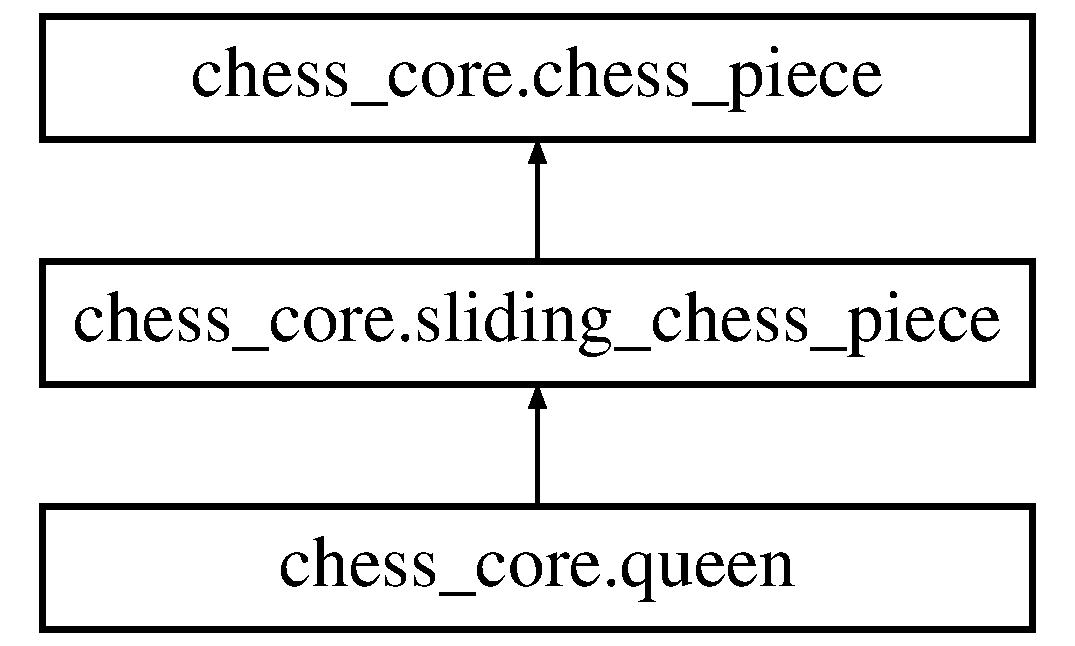
\includegraphics[height=3.000000cm]{classchess__core_1_1queen}
\end{center}
\end{figure}
\subsection*{Public Member Functions}
\begin{DoxyCompactItemize}
\item 
\hypertarget{classchess__core_1_1queen_ad308e56e5b4cb22ee9fb21ba990440ab}{}{\bfseries queen} (Point starting\+\_\+pos, \hyperlink{enumchess__core_1_1team__color}{team\+\_\+color} team, \hyperlink{classchess__core_1_1chess__game}{chess\+\_\+game} board)\label{classchess__core_1_1queen_ad308e56e5b4cb22ee9fb21ba990440ab}

\end{DoxyCompactItemize}
\subsection*{Additional Inherited Members}


\subsection{Detailed Description}
Created by tl on 2/11/15. Nothing interesting here, extends sliding chess piece 

The documentation for this class was generated from the following file\+:\begin{DoxyCompactItemize}
\item 
src/chess\+\_\+core/queen.\+java\end{DoxyCompactItemize}

\hypertarget{classchess__core_1_1rook}{}\section{chess\+\_\+core.\+rook Class Reference}
\label{classchess__core_1_1rook}\index{chess\+\_\+core.\+rook@{chess\+\_\+core.\+rook}}
Inheritance diagram for chess\+\_\+core.\+rook\+:\begin{figure}[H]
\begin{center}
\leavevmode
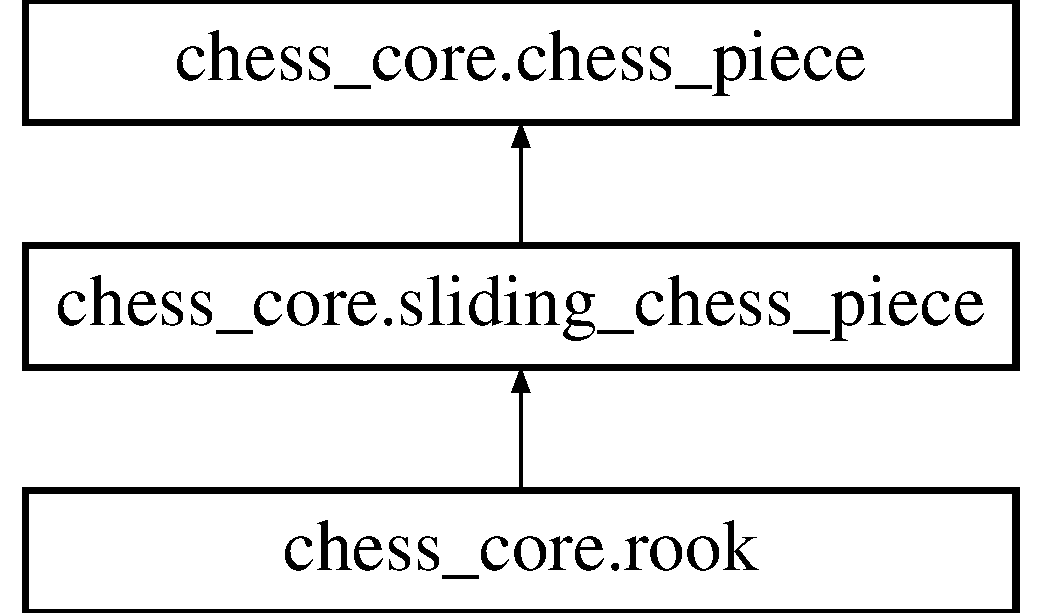
\includegraphics[height=3.000000cm]{classchess__core_1_1rook}
\end{center}
\end{figure}
\subsection*{Public Member Functions}
\begin{DoxyCompactItemize}
\item 
\hypertarget{classchess__core_1_1rook_a43e2fdb036efc12ba465107eeb10d6f3}{}{\bfseries rook} (Point starting\+\_\+pos, \hyperlink{enumchess__core_1_1team__color}{team\+\_\+color} team, \hyperlink{classchess__core_1_1chess__game}{chess\+\_\+game} board)\label{classchess__core_1_1rook_a43e2fdb036efc12ba465107eeb10d6f3}

\end{DoxyCompactItemize}
\subsection*{Additional Inherited Members}


\subsection{Detailed Description}
Created by tl on 2/11/15. Nothing interesting here, extends sliding chess piece 

The documentation for this class was generated from the following file\+:\begin{DoxyCompactItemize}
\item 
src/chess\+\_\+core/rook.\+java\end{DoxyCompactItemize}

\hypertarget{classchess__core_1_1sliding__chess__piece}{}\section{chess\+\_\+core.\+sliding\+\_\+chess\+\_\+piece Class Reference}
\label{classchess__core_1_1sliding__chess__piece}\index{chess\+\_\+core.\+sliding\+\_\+chess\+\_\+piece@{chess\+\_\+core.\+sliding\+\_\+chess\+\_\+piece}}
Inheritance diagram for chess\+\_\+core.\+sliding\+\_\+chess\+\_\+piece\+:\begin{figure}[H]
\begin{center}
\leavevmode
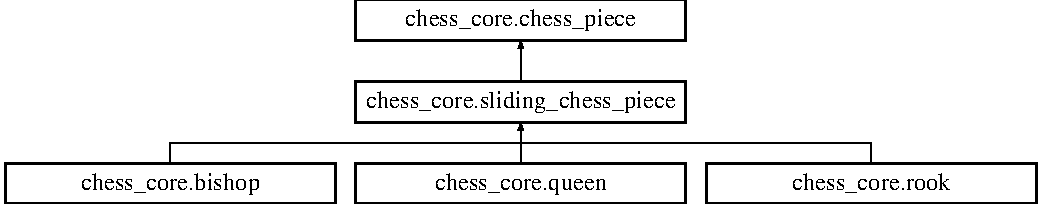
\includegraphics[height=2.745098cm]{classchess__core_1_1sliding__chess__piece}
\end{center}
\end{figure}
\subsection*{Public Member Functions}
\begin{DoxyCompactItemize}
\item 
\hypertarget{classchess__core_1_1sliding__chess__piece_a85cd8228689f00b73ecac63dd7daf714}{}{\bfseries sliding\+\_\+chess\+\_\+piece} (Point starting\+\_\+pos, \hyperlink{enumchess__core_1_1team__color}{team\+\_\+color} team, \hyperlink{classchess__core_1_1chess__game}{chess\+\_\+game} board)\label{classchess__core_1_1sliding__chess__piece_a85cd8228689f00b73ecac63dd7daf714}

\end{DoxyCompactItemize}
\subsection*{Protected Member Functions}
\begin{DoxyCompactItemize}
\item 
\hypertarget{classchess__core_1_1sliding__chess__piece_a9c6781ff5068ad3b4a6737b2732b9498}{}void {\bfseries update\+\_\+possible\+\_\+moves} ()\label{classchess__core_1_1sliding__chess__piece_a9c6781ff5068ad3b4a6737b2732b9498}

\end{DoxyCompactItemize}
\subsection*{Protected Attributes}
\begin{DoxyCompactItemize}
\item 
\hypertarget{classchess__core_1_1sliding__chess__piece_a76f45c6e7ad7e2d83d33a25ab0244813}{}Point\mbox{[}$\,$\mbox{]} {\bfseries movement\+\_\+vectors} = null\label{classchess__core_1_1sliding__chess__piece_a76f45c6e7ad7e2d83d33a25ab0244813}

\end{DoxyCompactItemize}


\subsection{Detailed Description}
Created by tl on 2/12/15.

A \char`\"{}\+Sliding\char`\"{} chess piece a sliding chess piece is allowed to move in a certain direction until it hits a wall or another piece Sliding pieces include pieces like \hyperlink{classchess__core_1_1rook}{chess\+\_\+core.\+rook} (moves horizontally and vertically), \hyperlink{classchess__core_1_1bishop}{chess\+\_\+core.\+bishop} (diagonal) and \hyperlink{classchess__core_1_1queen}{chess\+\_\+core.\+queen}

movement\+\_\+vectors = directions a sliding piece can move in with varying magnitudes incrementally tries movements in one direction until a wall is hit

To make a sliding chess piece, all that needs to be done is the movement\+\_\+vectors need to be defined 

The documentation for this class was generated from the following file\+:\begin{DoxyCompactItemize}
\item 
src/chess\+\_\+core/sliding\+\_\+chess\+\_\+piece.\+java\end{DoxyCompactItemize}

\hypertarget{classsquare__eight__chess_1_1square__eight__board}{}\section{square\+\_\+eight\+\_\+chess.\+square\+\_\+eight\+\_\+board Class Reference}
\label{classsquare__eight__chess_1_1square__eight__board}\index{square\+\_\+eight\+\_\+chess.\+square\+\_\+eight\+\_\+board@{square\+\_\+eight\+\_\+chess.\+square\+\_\+eight\+\_\+board}}
Inheritance diagram for square\+\_\+eight\+\_\+chess.\+square\+\_\+eight\+\_\+board\+:\begin{figure}[H]
\begin{center}
\leavevmode
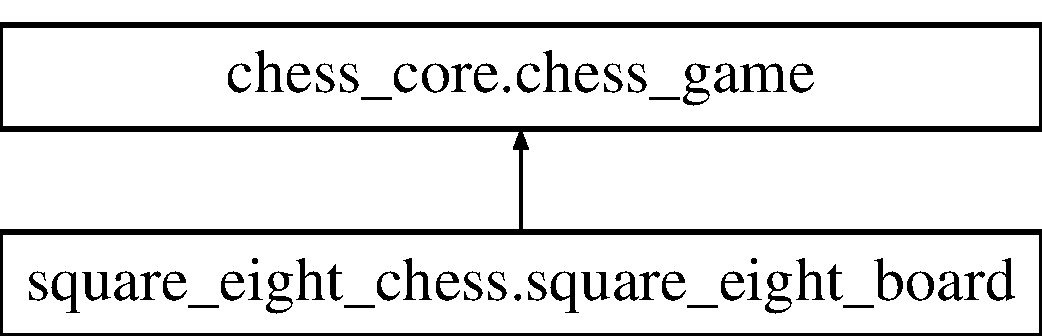
\includegraphics[height=2.000000cm]{classsquare__eight__chess_1_1square__eight__board}
\end{center}
\end{figure}
\subsection*{Public Member Functions}
\begin{DoxyCompactItemize}
\item 
\hypertarget{classsquare__eight__chess_1_1square__eight__board_a5e60ca24fedbd08797a902938b223405}{}void {\bfseries init\+\_\+game} ()\label{classsquare__eight__chess_1_1square__eight__board_a5e60ca24fedbd08797a902938b223405}

\item 
\hypertarget{classsquare__eight__chess_1_1square__eight__board_a8151b7261140f283d5221e391b0dbd17}{}boolean {\bfseries is\+\_\+in\+\_\+bounds} (Point position)\label{classsquare__eight__chess_1_1square__eight__board_a8151b7261140f283d5221e391b0dbd17}

\item 
\hypertarget{classsquare__eight__chess_1_1square__eight__board_a21dfcee69ba32ab3535d372958efbf4a}{}void {\bfseries init\+\_\+pawns} ()\label{classsquare__eight__chess_1_1square__eight__board_a21dfcee69ba32ab3535d372958efbf4a}

\item 
\hypertarget{classsquare__eight__chess_1_1square__eight__board_aeae9404b40adbb28830f63c9c0e547a5}{}void {\bfseries init\+\_\+queens} ()\label{classsquare__eight__chess_1_1square__eight__board_aeae9404b40adbb28830f63c9c0e547a5}

\item 
\hypertarget{classsquare__eight__chess_1_1square__eight__board_ad03c29d71fb7f063d0ad0a3379f57d08}{}void {\bfseries init\+\_\+kings} ()\label{classsquare__eight__chess_1_1square__eight__board_ad03c29d71fb7f063d0ad0a3379f57d08}

\item 
\hypertarget{classsquare__eight__chess_1_1square__eight__board_aa34b8eebcb3cabc26019f52d162bce5f}{}void {\bfseries init\+\_\+rooks} ()\label{classsquare__eight__chess_1_1square__eight__board_aa34b8eebcb3cabc26019f52d162bce5f}

\item 
\hypertarget{classsquare__eight__chess_1_1square__eight__board_a1c0b71070f453431c107c3c34d37c005}{}void {\bfseries init\+\_\+bishops} ()\label{classsquare__eight__chess_1_1square__eight__board_a1c0b71070f453431c107c3c34d37c005}

\item 
\hypertarget{classsquare__eight__chess_1_1square__eight__board_ad48cf674c92bdb3a90b845d1ba67e357}{}void {\bfseries init\+\_\+knights} ()\label{classsquare__eight__chess_1_1square__eight__board_ad48cf674c92bdb3a90b845d1ba67e357}

\end{DoxyCompactItemize}
\subsection*{Additional Inherited Members}


\subsection{Detailed Description}
Created by tl on 2/12/15. an implementation of a chess game -\/ the standard 8x8 chess game 

The documentation for this class was generated from the following file\+:\begin{DoxyCompactItemize}
\item 
src/square\+\_\+eight\+\_\+chess/square\+\_\+eight\+\_\+board.\+java\end{DoxyCompactItemize}

\hypertarget{classchess__core_1_1stepping__chess__piece}{}\section{chess\+\_\+core.\+stepping\+\_\+chess\+\_\+piece Class Reference}
\label{classchess__core_1_1stepping__chess__piece}\index{chess\+\_\+core.\+stepping\+\_\+chess\+\_\+piece@{chess\+\_\+core.\+stepping\+\_\+chess\+\_\+piece}}
Inheritance diagram for chess\+\_\+core.\+stepping\+\_\+chess\+\_\+piece\+:\begin{figure}[H]
\begin{center}
\leavevmode
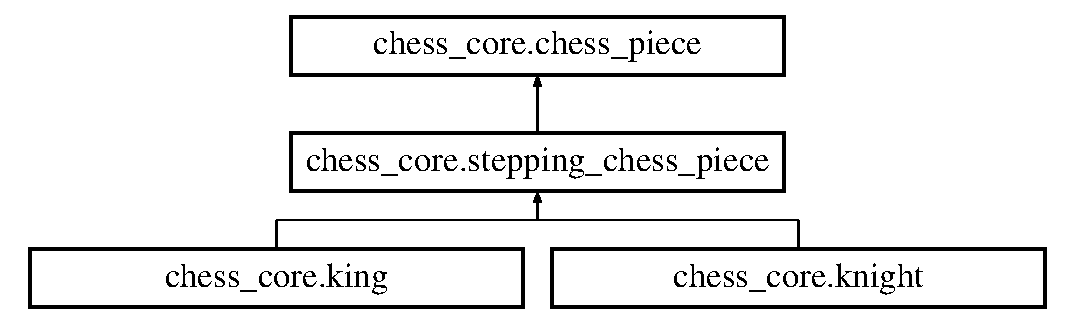
\includegraphics[height=3.000000cm]{classchess__core_1_1stepping__chess__piece}
\end{center}
\end{figure}
\subsection*{Public Member Functions}
\begin{DoxyCompactItemize}
\item 
\hypertarget{classchess__core_1_1stepping__chess__piece_a1c467ff3bf4e3107d7dc5788fa4563b8}{}{\bfseries stepping\+\_\+chess\+\_\+piece} (Point starting\+\_\+pos, \hyperlink{enumchess__core_1_1team__color}{team\+\_\+color} team, \hyperlink{classchess__core_1_1chess__game}{chess\+\_\+game} board)\label{classchess__core_1_1stepping__chess__piece_a1c467ff3bf4e3107d7dc5788fa4563b8}

\end{DoxyCompactItemize}
\subsection*{Protected Member Functions}
\begin{DoxyCompactItemize}
\item 
\hypertarget{classchess__core_1_1stepping__chess__piece_a6eac7103a31a0f5fab37455e1d23922a}{}void {\bfseries update\+\_\+possible\+\_\+moves} ()\label{classchess__core_1_1stepping__chess__piece_a6eac7103a31a0f5fab37455e1d23922a}

\end{DoxyCompactItemize}
\subsection*{Protected Attributes}
\begin{DoxyCompactItemize}
\item 
\hypertarget{classchess__core_1_1stepping__chess__piece_a52c2b3e29808226c7e0501e7821ac5b4}{}Point\mbox{[}$\,$\mbox{]} {\bfseries steps} = null\label{classchess__core_1_1stepping__chess__piece_a52c2b3e29808226c7e0501e7821ac5b4}

\end{DoxyCompactItemize}


\subsection{Detailed Description}
Created by tl on 2/12/15.

a \char`\"{}stepping\char`\"{} chess piece A piece that can step in certain directions, such as a \hyperlink{classchess__core_1_1knight}{chess\+\_\+core.\+knight} or a \hyperlink{classchess__core_1_1king}{chess\+\_\+core.\+king} steps = a table of moves a piece can make update\+\_\+possible\+\_\+moves() iterates through these steps and sees which are legal

To make a stepping class, just extend and fill in the steps table 

The documentation for this class was generated from the following file\+:\begin{DoxyCompactItemize}
\item 
src/chess\+\_\+core/stepping\+\_\+chess\+\_\+piece.\+java\end{DoxyCompactItemize}

\hypertarget{enumchess__core_1_1team__color}{}\section{chess\+\_\+core.\+team\+\_\+color Enum Reference}
\label{enumchess__core_1_1team__color}\index{chess\+\_\+core.\+team\+\_\+color@{chess\+\_\+core.\+team\+\_\+color}}
\subsection*{Public Attributes}
\begin{DoxyCompactItemize}
\item 
\hypertarget{enumchess__core_1_1team__color_a728984c7d43ed7ac493b3856d448cf94}{}{\bfseries White}\label{enumchess__core_1_1team__color_a728984c7d43ed7ac493b3856d448cf94}

\item 
\hypertarget{enumchess__core_1_1team__color_ae3478a6fb68ec863c54ab67bcb011c2d}{}{\bfseries Black}\label{enumchess__core_1_1team__color_ae3478a6fb68ec863c54ab67bcb011c2d}

\end{DoxyCompactItemize}


\subsection{Detailed Description}
Created by tl on 2/10/15. enums for team colors 

The documentation for this enum was generated from the following file\+:\begin{DoxyCompactItemize}
\item 
src/chess\+\_\+core/team\+\_\+color.\+java\end{DoxyCompactItemize}

%--- End generated contents ---

% Index
\backmatter
\newpage
\phantomsection
\clearemptydoublepage
\addcontentsline{toc}{chapter}{Index}
\printindex

\end{document}
